\documentclass[10pt]{article}

\usepackage{graphicx}
\usepackage{amsmath}
%\usepackage[ansinew]{inputenc}
\usepackage[utf8]{inputenc}
\usepackage[spanish]{babel}
\usepackage{babelbib}
\usepackage[T1]{fontenc}
\usepackage[vmargin=4cm,hmargin=4cm,letterpaper]{geometry}
\usepackage{color}
\usepackage{framed}
\usepackage{hyperref}
\usepackage{natbib}

\usepackage{listings}
\definecolor{red}{RGB}{219,0,0}
\definecolor{pink}{RGB}{255,100,100}
\definecolor{gray}{RGB}{100,100,100}
\lstset{
		basicstyle=\tiny,
		frame=single,
		keywordstyle=\color{red},
		commentstyle=\color{gray},
		stringstyle=\color{pink},
		tabsize=3,
		language=verilog,
		backgroundcolor=\color{white}}

\usepackage{fancyhdr} 
\pagestyle{fancy}
\usepackage{lastpage}
\lhead{Laboratorio 4 y Proyecto final}
\chead{}
\rhead{Bitácora}
\lfoot{}
\cfoot{}
\rfoot{\footnotesize Page \thepage\ of \pageref{LastPage}}

\renewcommand{\headrulewidth}{0.4pt} 
\renewcommand{\footrulewidth}{0.4pt} 

\graphicspath{{images/}}	%%multimedia path
\setlength{\parindent}{0pt}
%%*************************************************************************
\begin{document}

\begin{huge}
\begin{center}
\textbf{Proyecto : Snake World y Controlador VGA}
\end{center}
\end{huge}

\begin{Large}
\begin{center}
Jose Apú (B10407), Francisco Molina (B14194), \\Marco Montero (A94000), Dennis Vargas (B16831)
\end{center}
\end{Large}

\section{Objetivo General}

Desarrollar un controlador VGA utilizando una FPGA y posteriormente en la misma un juego de snake.\\[0.3 cm] \cite{papilio}

\subsection{Objetivos específicos}
\begin{itemize}
\item Utilizar los periféricos de la tarjeta de desarrollo.
\item Implementar diferentes módulos para cada parte del juego.
\item 
\end{itemize}

%%**********************************************************************
\section{Implementación}
Para la implementación el proyecto se puede separar en 3 módulos: el controlador VGA, el módulo que controla el mundo y el que controla el cuerpo y la cabeza de la serpiente. El controlador de VGA forma parte del laboratorio 4 del curso, consistió en imprimir en pantalla con la FPGA. Los otros 2 módulos forman parte del proyecto final, controlando tanto la lógica del juego como los colores que se quieren imprimir en cada pixel dependiendo de la misma lógica.
%%**************************************************
\subsection{Controlador VGA}

En primera instancia se desarrolló un controlador VGA encargado de desplegar datos en una pantalla, de forma que inicialmente se imprimió la pantalla en verde para comprobar su funcionamiento. Esta prueba y el juego se realizaron para una configuración de 640x480, para cuya sincronización se tomó como referencia la figura \ref{vga-data}.\\

\begin{figure}[hbtp]
\centering
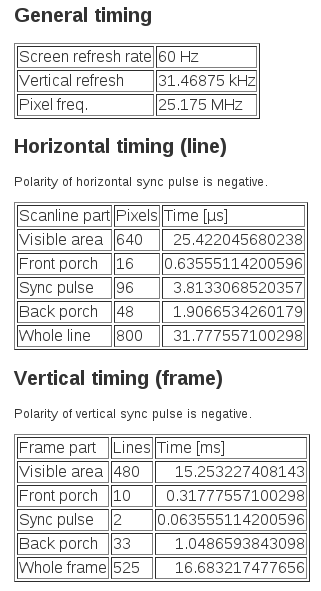
\includegraphics[width=0.4\textwidth]{vga-data.png}
\caption{VGA Signal 640 x 480 @ 60 Hz Industry standard timing}
\label{vga-data}
\end{figure}

Para este controlador es sumamente importante sincronizar las señales HSYNC y VYNC, verificar cuando se ponen en 0 y en 1, ya que estas controlan el reset vertical y horizontal. Para esto se tomó en cuenta el diagrama de la Figura \ref{vga-pulse}.\\

\begin{figure}[hbtp]
\centering
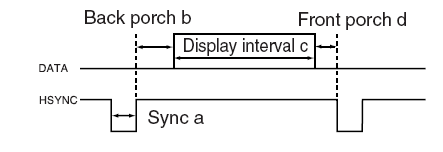
\includegraphics[width=0.4\textwidth]{vga-pulse.png}
\caption{Esquema de control}
\label{vga-pulse}
\end{figure}

Además es necesario tener dos contadores, uno para las filas y otro para las columnas, de forma que cuando llegue a un determinado valor se resetean el valor de los SYNCs y el de los contadores al valor inicial cero. Esta lógica se puede observar en el siguiente código:\\

\begin{lstlisting}
assign rowReset = (wRtemp == (WholeVFrame-1))? 1'b1:1'b0;
assign colReset = (wCtemp == (WholeHLine-1))? 1'b1:1'b0;

assign oVgaVsync = (wRtemp >= (VisibleVArea + FrontVPorch) && 
wRtemp <= (VisibleVArea + FrontVPorch + SyncVPulse))? 0:1;
assign oVgaHsync = (wCtemp >= (VisibleHArea + FrontHPorch) && 
wCtemp <= (VisibleHArea + FrontHPorch + SyncHPulse))? 0:1;
\end{lstlisting}

Una vez implementados los contadores, se ocupa un generador de señales, ya que tiene que se ocupa trabajar a una frecuencia determinada. Para eso se utilizó un DCM, de acuerdo con el siguiente código:

\begin{lstlisting}
DCM_SP # (
.CLKFX_MULTIPLY(25),	
.CLKFX_DIVIDE(32)		
)

ClockVga (
.CLKIN(Clock),			
.CLKFB(wVgaClock), 	
.RST( Reset ),			
.PSEN(1'b0), 			
.LOCKED(wPllLock),	//Para bloquear el Pll.
.PSDONE(wPsDone),	
.CLKFX(wVgaClock)		 
)
\end{lstlisting}

Por último se ocupan los valores RGB, los que definen el color del pixel. Para lo designado en el laboratorio 4, la prueba inicial consistió en únicamente desarrollar el controlador, para la cual se definieron valores fijos para todos los pixeles. Para el juego, estos datos se controlaron con los otros módulos.


%%**************************************************
\subsection{El mundo}
El módulo mundo define el área de juego y la comida que va apareciendo de manera aleatoria. Si bien crear datos aleatorios no es algo trivial, podríamos hablar de generar datos pseudoaleatorios. Para esto se utilizó el siguiente código:

\begin{lstlisting}
always @(iPixelRow,iPixelCol) 
begin		
	rLocationXTemp = ((x + 4271)*4273 - 9973*3)*57;
	rLocationYTemp = ((y + 3343)*3347 - 9857*3)*55;
	x = rLocationXTemp;
	y = rLocationYTemp;
end
\end{lstlisting}

$X$ y $Y$ toman un valor inicial e irá cambiando indefinidamente con la ecuación anterior. Con estos dos valores se elige la posición de la próxima comida cada vez que la serpiente se la come. Los valores de rLocationXTemp, rLocationYTemp, $x$, $y$, son números de 8 bits, por lo que nunca serán más grandes de 256 (el mundo es de 256x256) y siempre estarán adentro del área del mundo.\\
Una vez obtenida la posición aleatoria en un recuadro, se utiliza el siguiente código para colocar la comida, sumando los valores 192 y 112 para centrar este recuadro con el área de juego:

\begin{lstlisting}
begin
		oFoodLocationX = rLocationXTemp + 11'd192;
		oFoodLocationY = rLocationYTemp + 11'd112;
end
\end{lstlisting}

%%**************************************************
\subsection{La serpiente}

El módulo serpiente se divide en tres submódulos. El primero llamado SnakeIcon genera la serpiente, SnakeMovement se encarga de controlar el movimiento y por último SnakeMain une estos dos módulos.

\subsubsection{SnakeIcon}

La serpiente se forma por un arreglo de cuadros (pixeles). En un inicio cuenta con 25 cuadros y puede llegar a un máximo de 100.\\

Cuando la serpiente come, el cuadro nuevo adopta el valor del cuadro anterior. De forma que si al comer, la serpiente actualmente es de 30 cuadros, el cuadro 31 pasa a ser el cuadro 30, el 30 pasa hacer el 29 y así sucesivamente hasta llegar al cuadro cero que toma el valor de la comida.\\

Este submódulo también se encarga de verificar si uno pierde la partida, ya sea si se tocó así mismo o toco una pared.

\begin{lstlisting}
//Cuando toca una pared
		if (oSnakeLenght >= 8'd26 || iLocationX <= 11'd192 ||  
		                             iLocationX >= 11'd449 || 
		                             iLocationY <= 11'd112 || 
		                             iLocationY >= 11'd368)
			oGameOver = 1;
		else
			oGameOver = 0;

//Cuando se come asi mismo			
		for(j=100;j>=2;j=j-1) 
		begin
			//revisa si la cabeza tiene un valor igual a alguno del cuerpo 
			if(rBodyStack[0] == rBodyStack[j] && j <= oSnakeLenght)
				oGameOver = 1;
			else
				oGameOver = oGameOver;
		end	
\end{lstlisting}
		 
\subsubsection{SnakeMovement}
Este submódulo se encarga de cambiar el estado de dirección ya sea North, South, West o East. Estos estados se cambian al darle click a cualquiera de los cuatro botones de la papilio. Por ejemplo si se da click al boton de arriba el estado cambia a North, si estaba en North lo mantiene.

\begin{lstlisting}
always @(*)
begin
	if(iWest == 1'b1)
		rUserInput = `West;
	else if(iEast == 1'b1)
		rUserInput = `East;
	else if(iSouth == 1'b1) 
		rUserInput = `South;
	else if(iNorth == 1'b1)
		rUserInput = `North;
	else	
		rUserInput = rUserInput;
end
\end{lstlisting}

Adicionalmente se controla la velocidad y lo más importante, el movimiento. Dependiendo del estado con cada nivel se va agregando velocidad a la serpiente. Es importante aclarar que no se puede cambiar el sentido drásticamente, es decir no se puede pasar del estado North a South en un mismo movimiento, por lo que también se controla este tipo de restricciones. Esto último se implementa de la siguiente manera:

\begin{lstlisting}
if(rUserInput == `West && rCurrentHeading != `West && rCurrentHeading != `East)
			rCurrentHeading = `West;

		else if(rUserInput == `East && rCurrentHeading != `West && rCurrentHeading != `East)
			rCurrentHeading = `East;

		else if(rUserInput == `North && rCurrentHeading != `North && rCurrentHeading != `South)
			rCurrentHeading = `North;

		else if(rUserInput == `South && rCurrentHeading != `North && rCurrentHeading != `South)
			rCurrentHeading = `South;
		else
			rCurrentHeading = rCurrentHeading;
\end{lstlisting}

\subsubsection{SnakeMain}
Este submódulo se encarga de instanciar los dos anteriores, por cuestión de orden y facilidad para despulgar.

%%**********************************************************************
\section{Resultados}

\begin{figure}[hbtp]
\centering
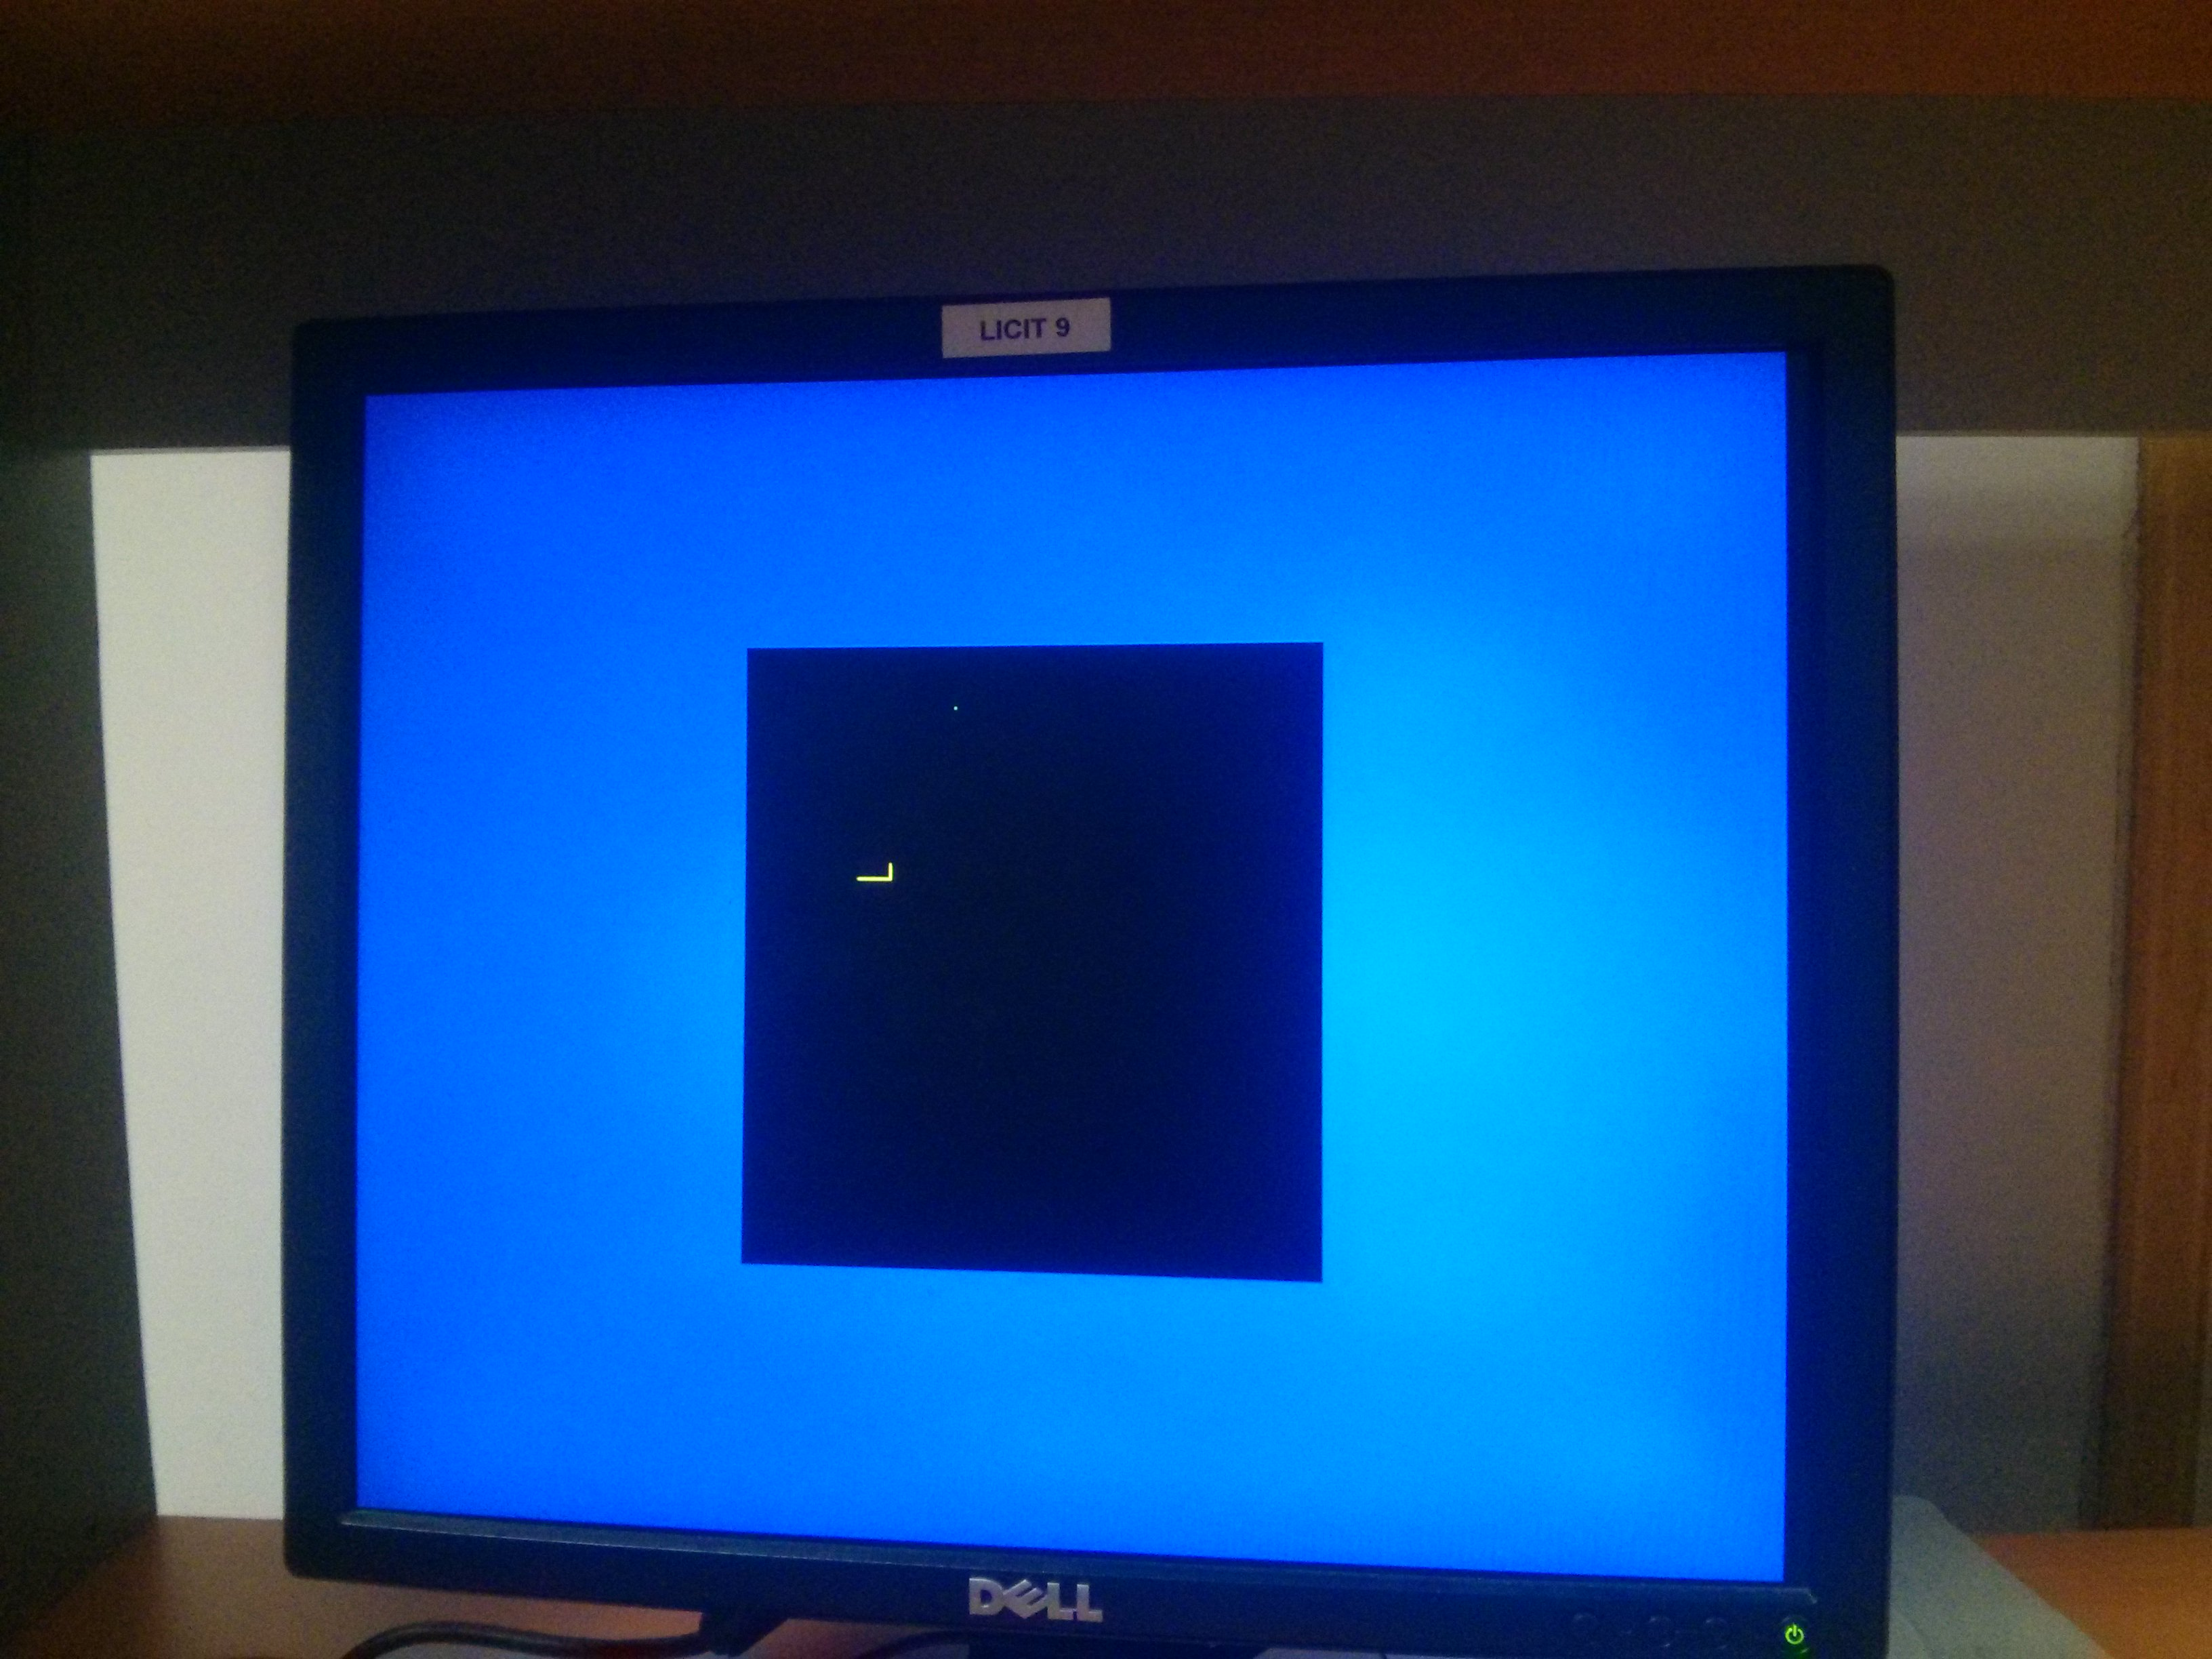
\includegraphics[width=1\textwidth]{game-play}
\caption{Game play}
\label{vga-play}
\end{figure}

\begin{figure}[hbtp]
\centering
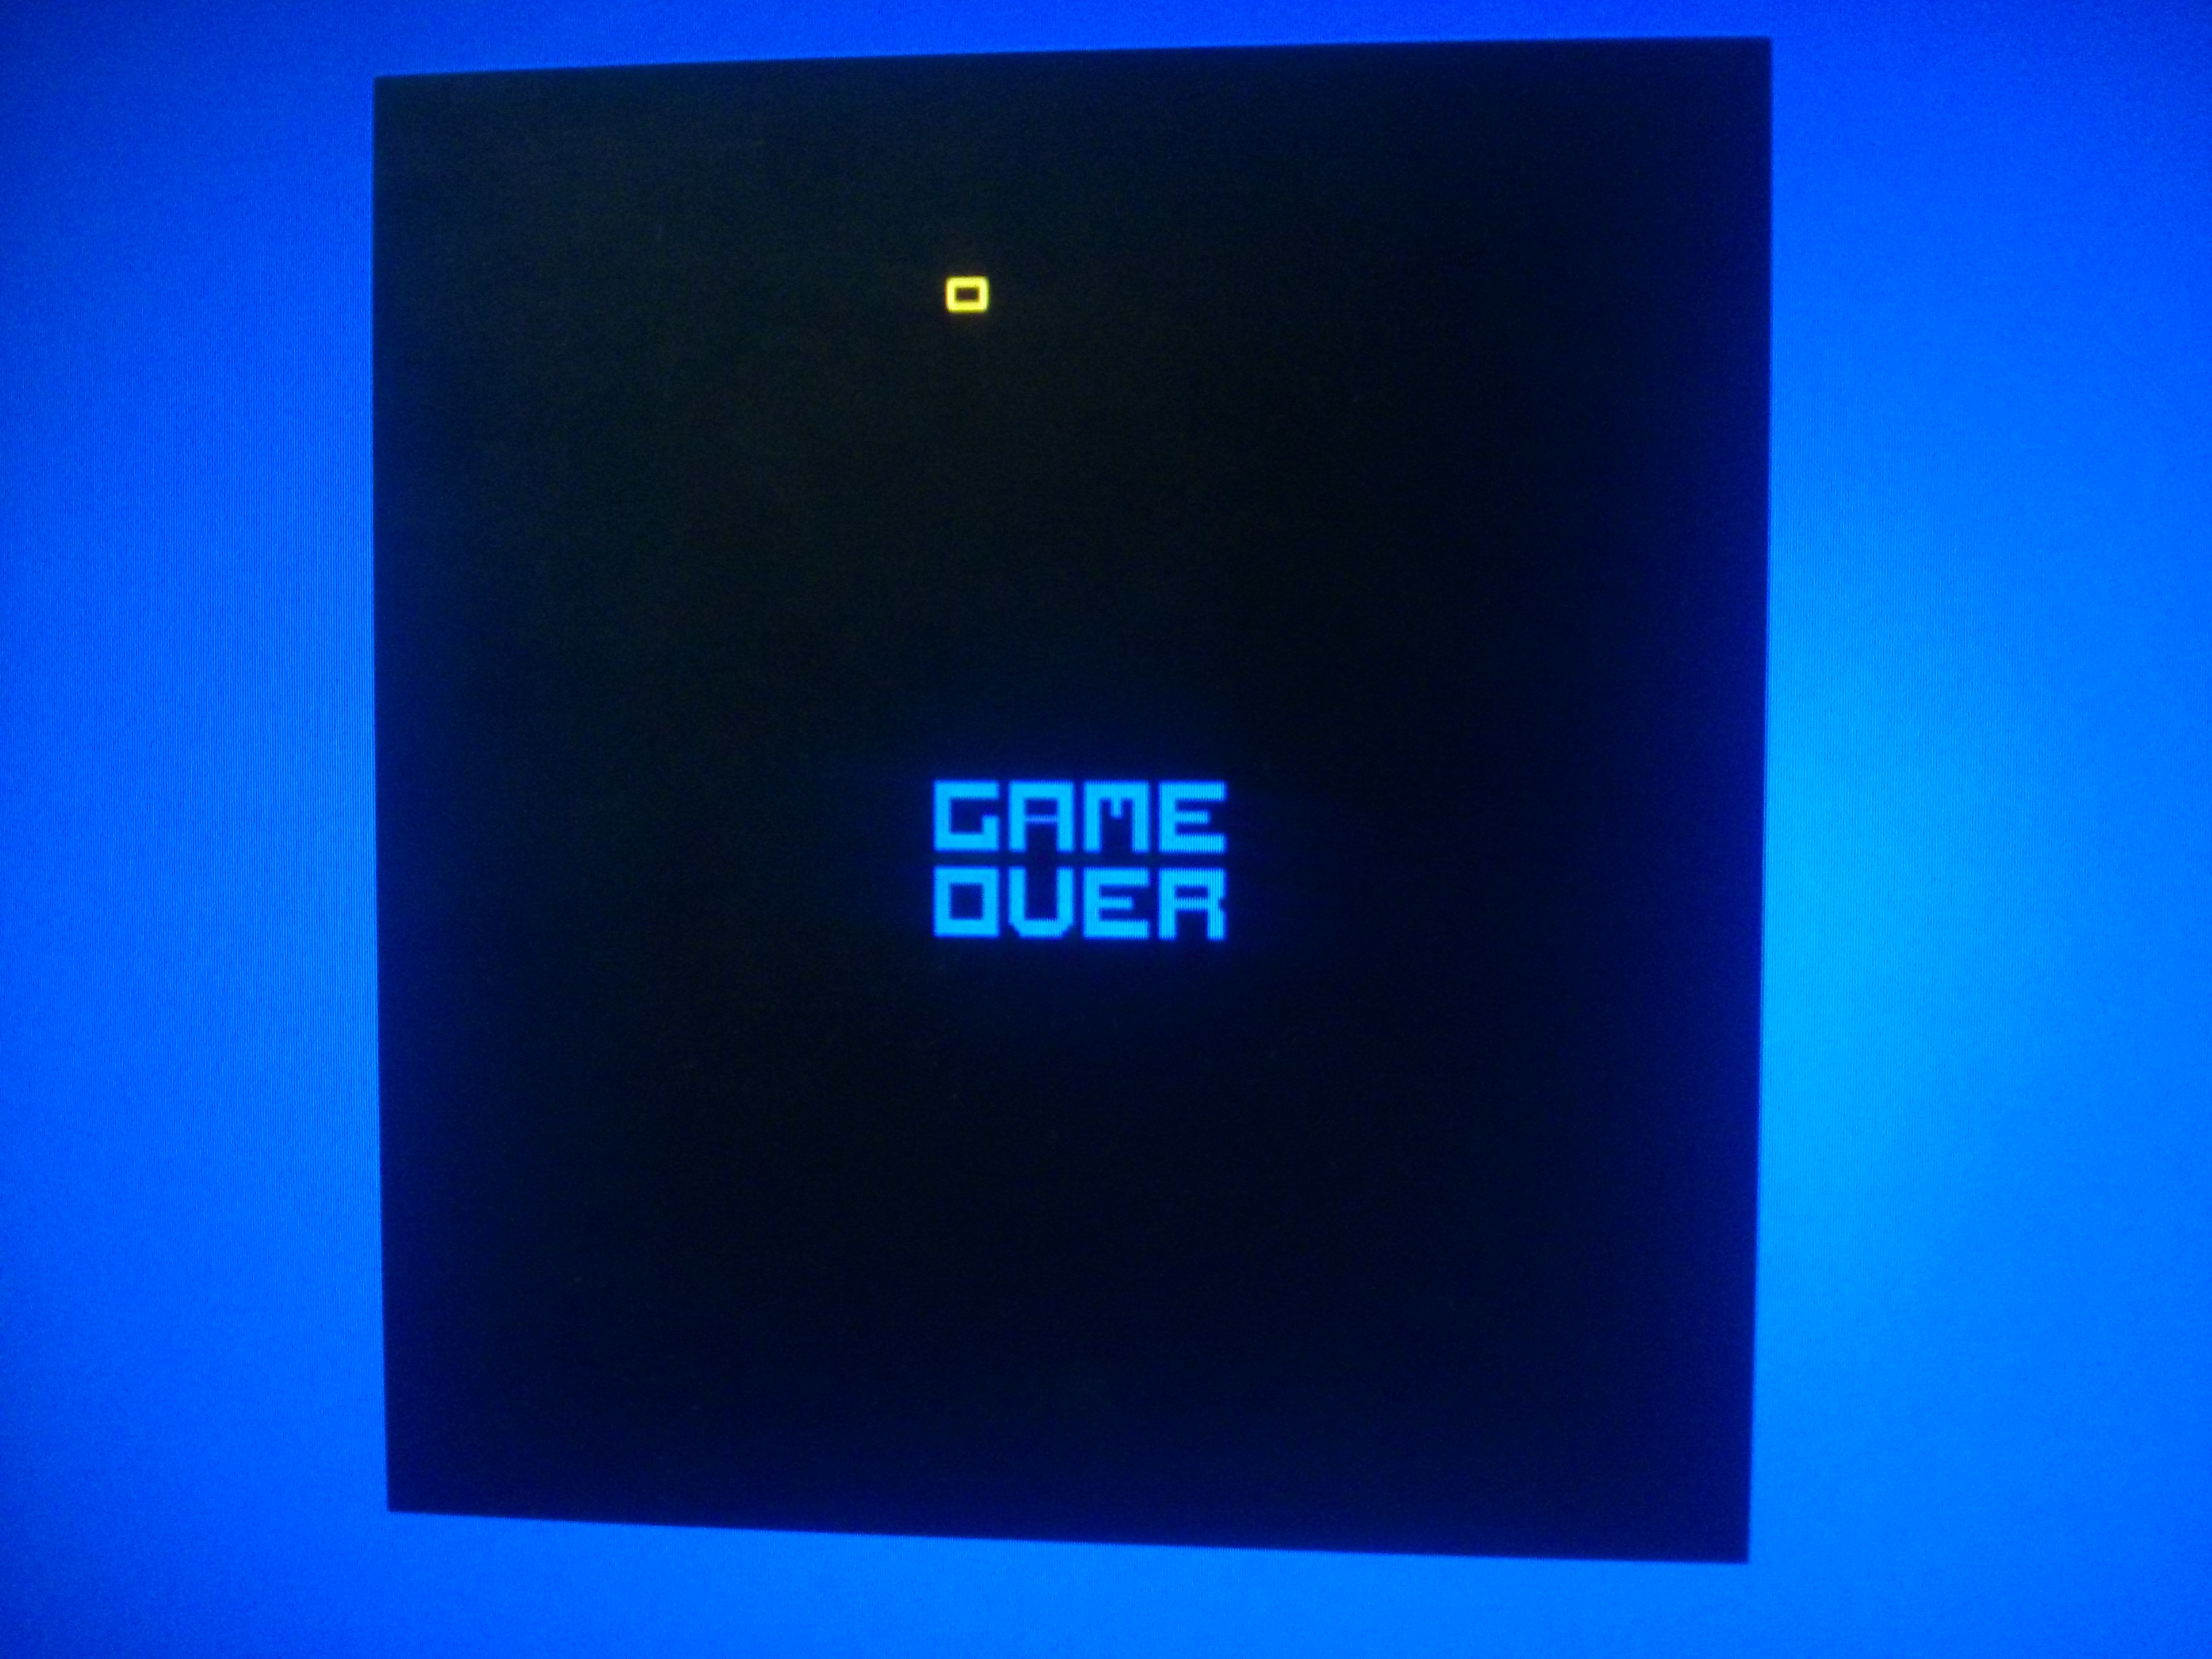
\includegraphics[width=1\textwidth]{game-over}
\caption{Game over tocandose así mismo}
\label{vga-over}
\end{figure}

\begin{figure}[hbtp]
\centering
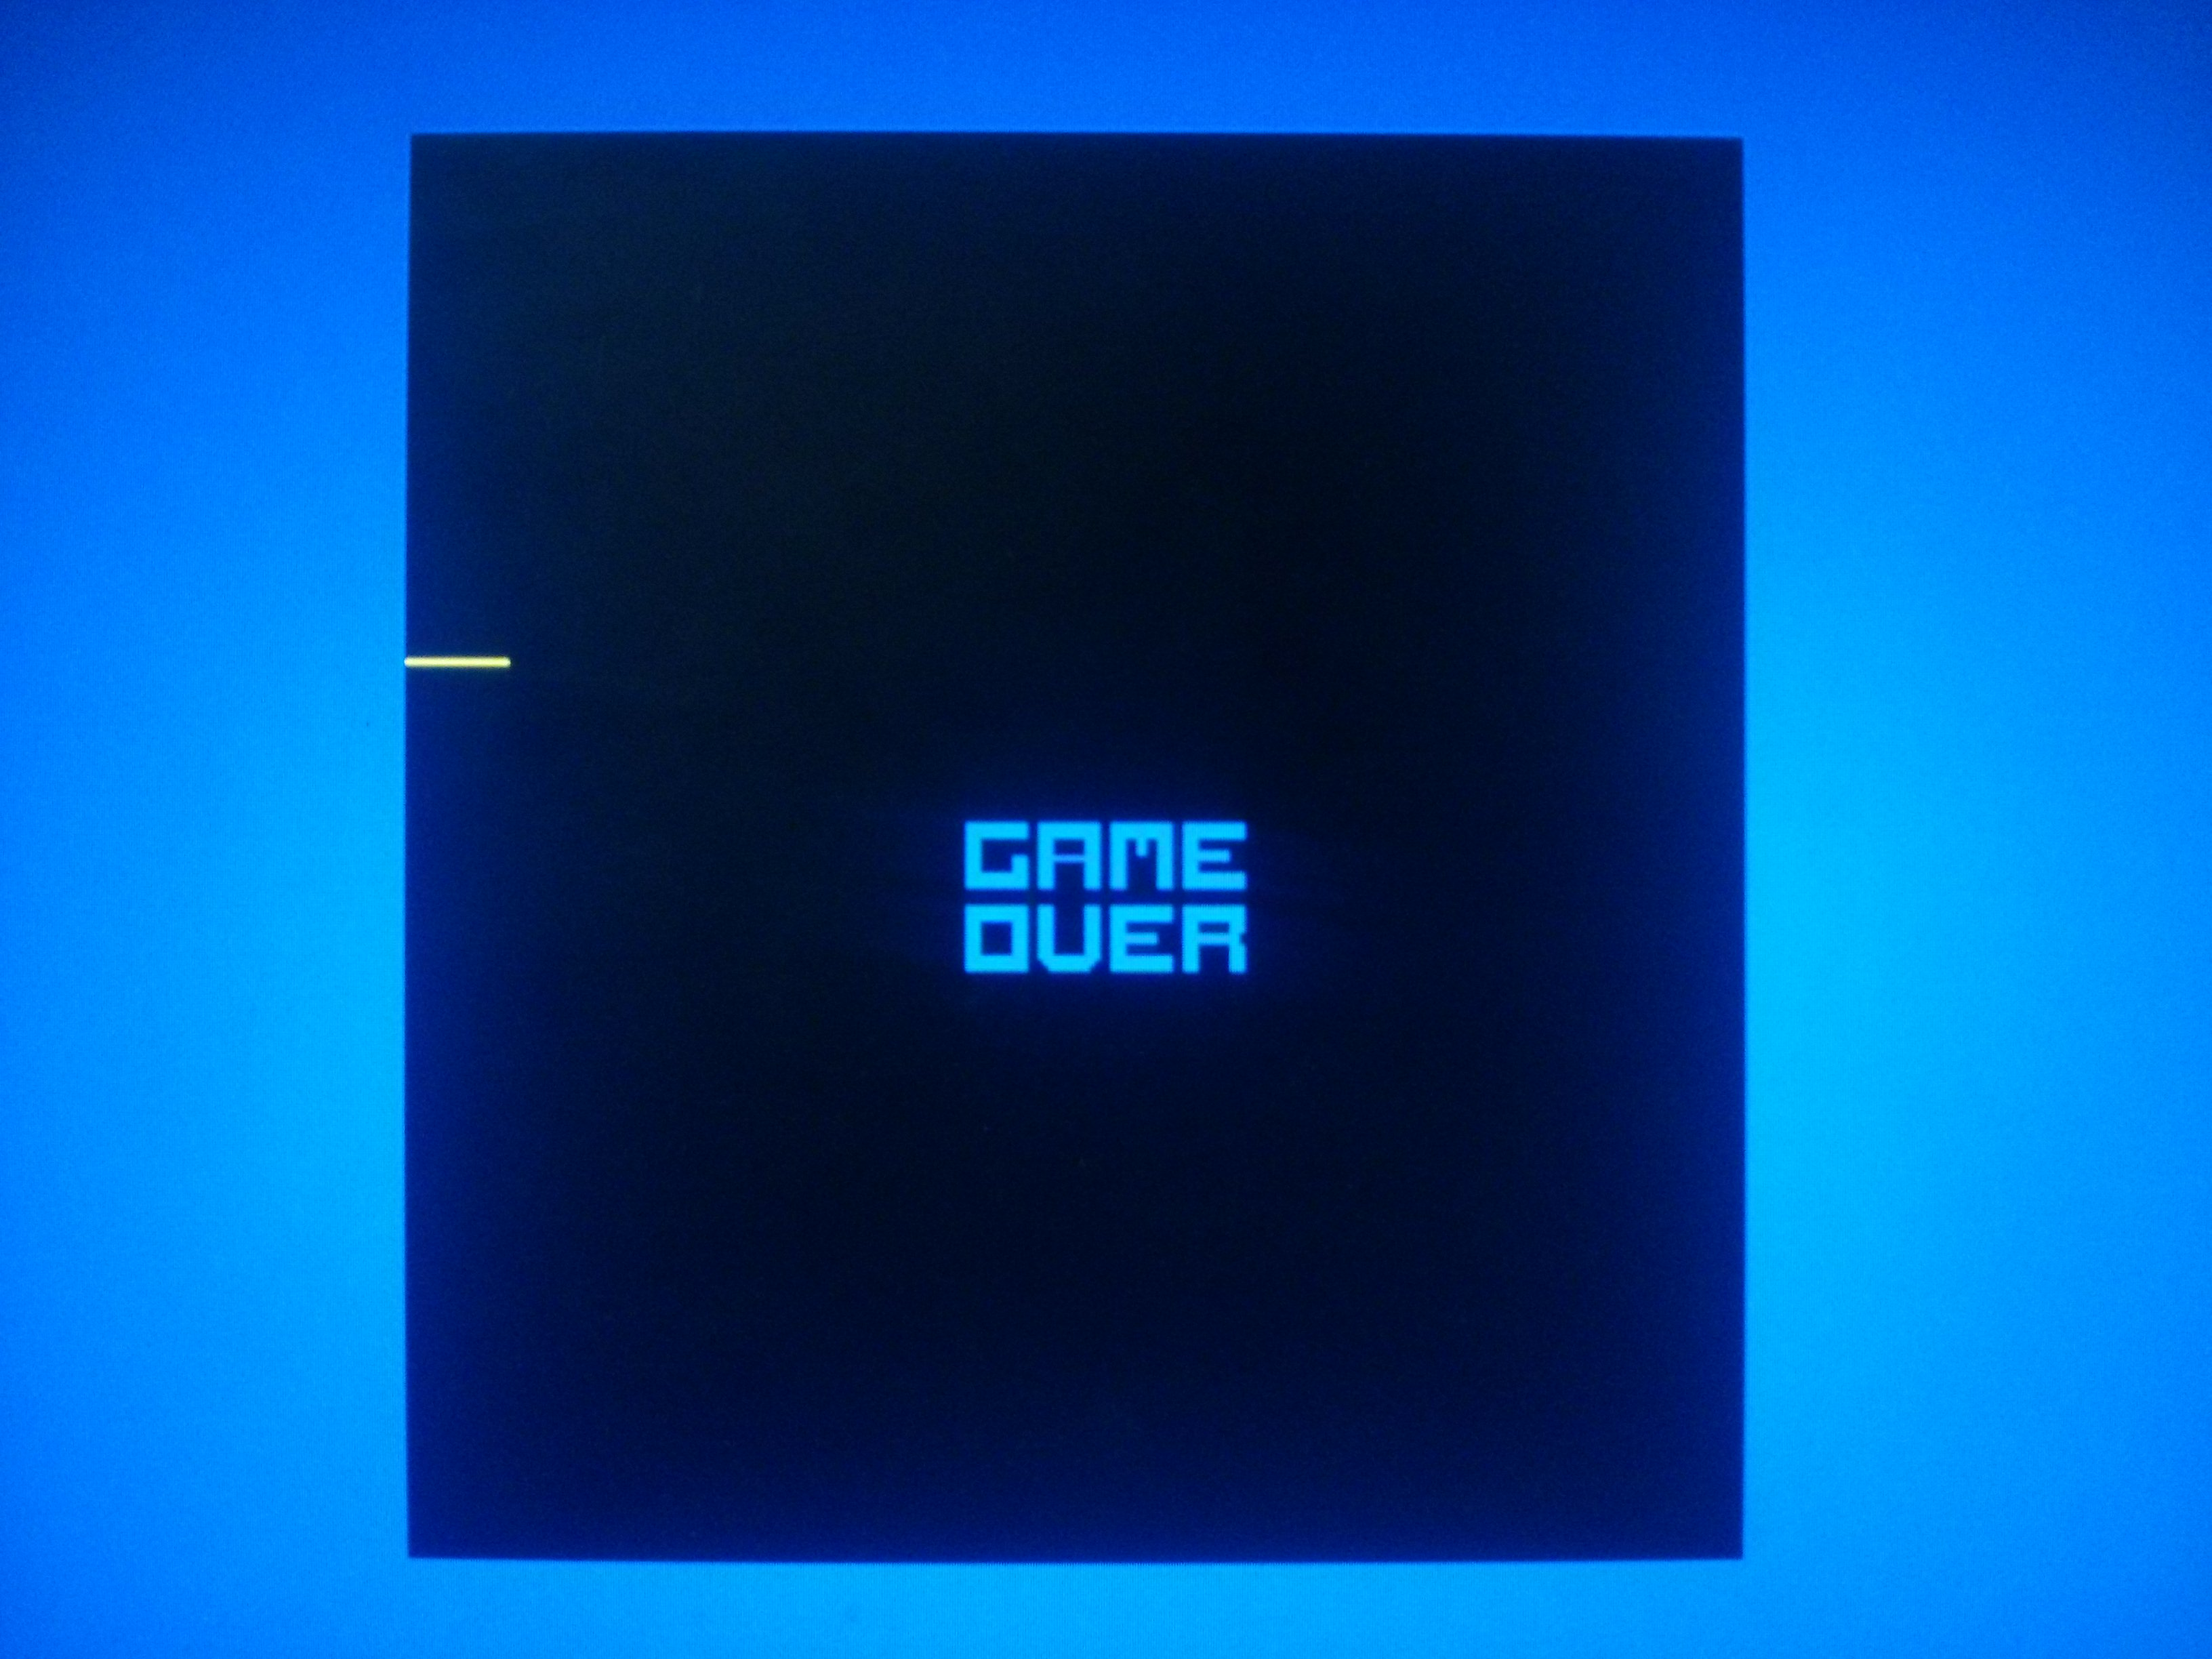
\includegraphics[width=1\textwidth]{game-over-side}
\caption{Game over tocando un lado}
\label{vga-over-side}
\end{figure}

%%**********************************************************************
\section{Discusión}
En cuanto al módulo de controlador de VGA el principal problema fue la sincronización de las señales Hsync y Vsync. Ya que para que la pantalla reconozca la comunicación se necesita "hablar" con la misma de forma que las señales cumplan la temporización respectiva. \\
Para el desarrollo del juego, una vez implementado, se notó que la posición de la comida aparecía algunas veces fuera del rango del mundo, esto ya que no se había centrado el recuadro para calzar con el área de juego, lo cuál arregló el bug.\\
Como futuras recomendaciones, al ser la serpiente de un pixel de grosor, es díficil para el usuario el control de misma, de forma que se propone ensanchar la serpiente para tener una mejor experiencia de juego. 
%%**********************************************************************
\section{Conlusiones}
Desarrollar un proyecto conlleva una mayor dificultad que un laboratorio, para interés del curso se cumplió con las expectativas y los objetivos planteados, ampliando los conocimientos teóricos y prácticos en cuanto a la materia de circuitos digitales. El realizar el juego snake no sólo consistió en la aplicación de los laboratorios anteriores, sino también en la implementación como equipo de una estrategia de modularización para conllevar un proyecto en conjunto, desarrollando el código paso a paso y arreglando basados en aportes de cada uno los diferentes problemas como la sincronización de las señales y la posición aleatoria de la comida. \\
Realizar en una FPGA proyectos a nivel académico aporta sumamente al entendimiento de los circuitos digitales, así como a su aplicación en la vida real y la forma en que se han desarrollado proyectos a nivel comercial.

%%**********************************************************************
\bibliography{bitacora}
\bibliographystyle{abbrv}
\end{document}
%%*************************************************************************
